\section{Introduction}
\label{sec:intro}

The product of mesh-to-CAD reconstruction is a program. A designer edits its sketches and features, and a CAD kernel turns it into a solid. Optimization-based reconstructors such as CADFit \citep{nehme2026cadfit} build that program by proposing extrusions and revolves fitted to slices of the target mesh, composing them with booleans, and keeping the composition with the highest volumetric IoU. In practice the score that steers and reports the search is computed on meshes: candidate solids are tessellated, combined with mesh booleans, and compared with the target. The program assembled at the end is a separate artifact. Whether it builds, whether the kernel accepts it, and whether it reproduces the reported geometry are not part of the number.

This gap matters more as search gets stronger. A search that explores more compositions has more chances to find meshes whose program cannot be replayed, and a measurement error that favours some candidates changes which compositions win. It also matters for the recent wave of LLM agents for CAD \citep{mallis2025cadassistant,savrasov2026cadfather}, which give a language model geometric tools and report reconstruction quality. CADFather \citep{savrasov2026cadfather} ablates its tools but leaves open how much of an agent's result comes from the tools and how much from the model's choices among them. Answering that requires a non-LLM policy over the same tools and budget, and a metric that cannot be gamed by unexecutable output.

We study three questions on a cohort of \nFresh{} hard-tier CADBench parts \citep{doris2026cadbench} drawn after, and disjoint from, every part used during development:
\begin{itemize}
\item[\textbf{Q1}] Does mesh IoU track the IoU of the executed program (\iouc) as the search gets stronger?
\item[\textbf{Q2}] Which search extensions improve the executed program, not just the reported mesh?
\item[\textbf{Q3}] Do the optimizer's own stages make open-weight LLMs competent CAD agents, and does the LLM add anything over a script that uses the same stages?
\end{itemize}

\begin{figure}[t]
\centering
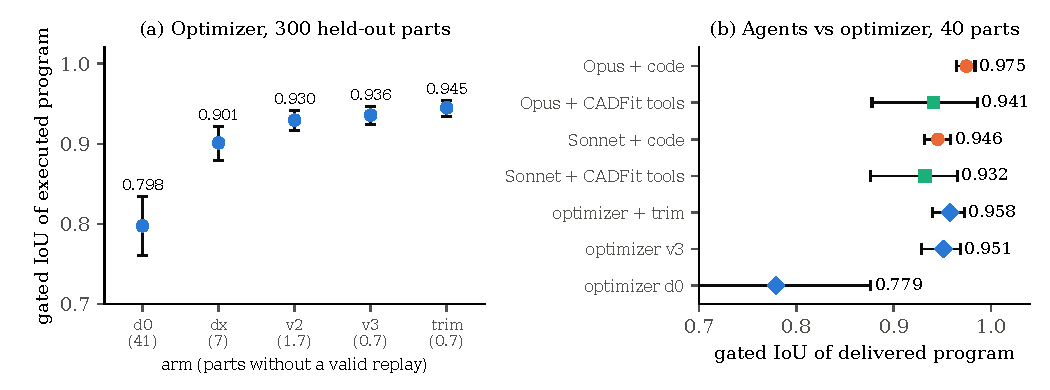
\includegraphics[width=\linewidth]{figures/hero.pdf}
\caption{\textbf{(a)} Search arms on \nFresh{} fresh parts. Light bars score the mesh the search reports; dark bars score the solid built by executing the final program. Error bars: 95\% bootstrap intervals of the mean over parts. Red: unbuilt + OCC-invalid programs; n/m = validity not measured for the best-of control. \textbf{(b)} Six open-weight agents on \nAgentParts{} of those parts, writing CadQuery alone (open) or with CADFit stages as tools (filled); failed episodes score 0. Vertical lines: the strongest pipeline arm on the same parts and two scripted policies over the same tools; the unrestricted one is labelled with its free ground-truth trials.}
\label{fig:hero}
\end{figure}

Our answers, summarised in \cref{fig:hero}:
\begin{enumerate}
\item \textbf{Execution changes the ranking of search extensions} (\cref{sec:search}). The gap between mesh IoU and \iouc{} grows from the base pipeline (\armBaseGap) to beam search (\armBeamGap), almost entirely through programs that do not build. Gains in \iouc{} are measurably smaller than gains in mesh IoU for the rule package and for the full ladder of extensions. We also document measurement defects in the stock objective and judge, including an alpha-wrapped objective, cavity filling and self-intersecting lofts, that change individual scores (\cref{sec:measure}).
\item \textbf{Whole-part section proposals survive execution} (\cref{sec:search}). Adding a mid-plane section extrusion per axis to the candidate pool is the largest observed \iouc{} increment among our extensions (\dSecBeamCadDiff, 95\% interval \dSecBeamCadCI). The gain is concentrated on benchE; over the corrected base pipeline the overall \iouc{} gain is not established.
\item \textbf{Optimizer stages are effective tools for open-weight agents} (\cref{sec:agents}). With the stages as tools, all six models improve over writing CadQuery alone, by \skillsGainMin{} to \skillsGainMax{} \iouc{}, and every Bonferroni-corrected interval excludes zero. The best agent's mean is \mGemmaVsPipeDiff{} relative to the strongest pipeline arm on the same parts (interval \mGemmaVsPipeCI). A scripted policy with the same tools and budget is not shown to be worse than any agent.
\end{enumerate}

The evaluation protocol, the extensions, the agent harness and every script that regenerates our tables are released with the paper.
